\documentclass[12pt,oneside]{book}
\newcommand{\TITLE}{Statistique}
\usepackage[utf8]{inputenc}
\usepackage[margin=0.5in]{geometry}
\usepackage[usestackEOL]{stackengine}
\usepackage{amsmath , esint,braket,lmodern,mhchem,bohr,lewis,chemfig,draftwatermark,xcolor,graphicx , amssymb ,ragged2e , listings , siunitx , float , eqparbox, centernot , esvect , bm , fancyhdr , fourier-orns}
\usepackage[ddmmyyyy]{datetime}
\usepackage{fourier-orns}
\usepackage{changepage}
\usepackage{bbm}\usepackage{chngcntr}
\usepackage{hyperref}
\usepackage{ifthen}
\usepackage[many]{tcolorbox}
\DeclareMathOperator{\sech}{sech}
\DeclareMathOperator{\csch}{csch}
\DeclareMathOperator{\arcsec}{arcsec}
\DeclareMathOperator{\arccot}{arcCot}
\DeclareMathOperator{\arccsc}{arcCsc}
\DeclareMathOperator{\arccosh}{arcCosh}
\DeclareMathOperator{\arcsinh}{arcsinh}
\DeclareMathOperator{\arctanh}{arctanh}
\DeclareMathOperator{\arcsech}{arcsech}
\DeclareMathOperator{\arccsch}{arcCsch}
\DeclareMathOperator{\arccoth}{arcCoth} 
\DeclareMathOperator{\grad}{\vv{\text{grad}}} 
\DeclareMathOperator{\conj}{^*} 
\DeclareMathOperator{\vect}{vv} 
\DeclareMathOperator{\Vect}{\text{Vect}} 
\DeclareMathOperator{\degree}{c^\circ} 
\DeclareMathOperator{\degre}{^\circ} 
\DeclareMathOperator{\transpose}{^\dagger} 
\DeclareMathOperator{\adjoint}{^\dagger} 

\newcommand{\moyenne}[1]{\langle #1 \rangle} 
\newcommand{\lagrange}{\mathcal{L}}
\newcommand{\fourier}{\mathcal{F}}
\newcommand{\hilbert}{\mathcal{H}}
\newcommand{\p}{\mathcal{P}}
\newcommand{\x}{\chi}
\newcommand{\ve}[1]{\vv{#1}}
\newcommand{\push}[1]{\begin{adjustwidth}{5mm}{}#1\end{adjustwidth}}
\newcommand{\operator}[1]{\widehat{#1}}
\newcommand{\HRule}{\rule{\linewidth}{0.5mm}} % Defines a new command for the horizontal lines, change thickness here
\renewcommand{\chaptermark}[1]{\markboth{\MakeUppercase{#1}}{}}
\renewcommand{\headrule}{%
\vspace{-8pt}\hrulefill
\raisebox{-2.1pt}{\quad\decofourleft\decotwo\decofourright\quad}\hrulefill}
\definecolor{myred}{RGB}{255, 14, 0}
\everymath{\displaystyle}

\def\changemargin#1{\list{}{\leftmargin#1}\item[]}
\let\endchangemargin=\endlist 

\makeatletter
\newcommand*{\rom}[1]{\expandafter\@slowromancap\romannumeral #1@}%roman numbers
\makeatother

%hyperlink shit

\hypersetup{
    colorlinks,
    citecolor=black,
    filecolor=black,
    linkcolor=black,
    urlcolor=black
}
% Table specail cell , it's for making line break in table cell
\newcommand{\specialcell}[2][c]{%
  \begin{tabular}[#1]{@{}c@{}}#2\end{tabular}}

  \definecolor{main}{HTML}{5989cf}    % setting main color to be used
\definecolor{sub}{HTML}{cde4ff}     % setting sub color to be used

\tcbset{
    sharp corners,
    colback = white,
    before skip = 0.2cm,    % add extra space before the box
    after skip = 0.5cm      % add extra space after the box
}   
\newtcolorbox{boxH}{
    colback = sub, 
    colframe = main, 
    boxrule = 0pt, 
    leftrule = 6pt % left rule weight
}
\newtcolorbox{gpt}{
    sharpish corners, % better drop shadow
    boxrule = 0pt,
    toprule = 4.5pt, % top rule weight
    enhanced,
    fuzzy shadow = {0pt}{-2pt}{-0.5pt}{0.5pt}{black!35} % {xshift}{yshift}{offset}{step}{options} 
}
\definecolor{codegreen}{rgb}{0,0.6,0}
\definecolor{codegray}{rgb}{0.5,0.5,0.5}
\definecolor{codepurple}{rgb}{0.58,0,0.82}
\definecolor{backcolour}{rgb}{0.95,0.95,0.92}

\lstdefinestyle{mystyle}{
    backgroundcolor=\color{backcolour},   
    commentstyle=\color{codegreen},
    keywordstyle=\color{magenta},
    numberstyle=\tiny\color{codegray},
    stringstyle=\color{codepurple},
    basicstyle=\ttfamily\footnotesize,
    breakatwhitespace=false,         
    breaklines=true,                 
    captionpos=b,                    
    keepspaces=true,                 
    numbers=left,                    
    numbersep=5pt,                  
    showspaces=false,                
    showstringspaces=false,
    showtabs=false,                  
    tabsize=2,
    basicstyle = \small
}

\lstset{style=mystyle}
\SetWatermarkAngle{45} 
\SetWatermarkLightness{.99} 
\SetWatermarkFontSize{0.1cm} 
\SetWatermarkScale{0} 
\SetWatermarkText{supahaka}


\begin{document}
\pagestyle{fancy}
\fancyhf{}
\fancyfoot[R]{Tenji$_\text{org}$}
\fancyfoot[C]{\thepage}
\fancyfoot[L]{\tiny www.tenji.org}
\fancyhead[RO]{\nouppercase{\leftmark\hfill\TITLE}}


\DraftwatermarkOptions{stamp=false}
    \begin{titlepage}
        \begin{center}
            \vspace*{5cm}
            \Huge
            \HRule \\[0.4cm]
            \textbf{Project Tenji: \\ \TITLE}\\
            \Large 
            \HRule \\[1.5cm]
            \vspace{2cm}
            \vfill
        \end{center}
        \vfill
        { \scriptsize Project Tenji \copyright 2024 by Khalil Salahat and Mohamad El Moussawi  \\}
        { \scriptsize Hosted at tenji.org , contact : contact@tenji.org \\}
        { \scriptsize \NOTICEE  \\}
    \end{titlepage} 
    \tableofcontents
\DraftwatermarkOptions{stamp=true}


\chapter{RAPPELS DE THERMODYNAMIQUE}
Le thermodynamique est la branche de la physique dont le principal but est de décrire les transformations entre le deux formes d'énergie le travail et la chaleur. C'est une science qui s'applique aux corps macroscopiques.
\section{Definitions}
\subsection{Système}
On appelle système une partie de l'univers entourée par une surface fermée.\\
Un système est isolé (ou fermé) s'il n'a pas d'interaction avec le reste de l'univers.\\
Il est ouvert dans le cas contraire.\\

Un système est homogène si, en l'absence de champ extérieur, la concentration de ses constituants est la même en tout point.\\
Dans le cas contraire il est dit hétérogène.
\subsection{État macroscopique}
Nous appellerons état macroscopique ou macro-état la configuration qui est associée à la valeur des paramètre qui décrites les propriétés thermodynamiques d'un système, ce sont par exemple :
\begin{itemize}
	\item La température absolue $T$.
	\item La pression $P$.
	\item le nombre de particules $N$.
\end{itemize}
L'equation d'état des gaz parfaits :
\[PV = nRT\]
\subsection{Thermomètre}
Un thermomètre est un petit système permettant de mesurer la température d'un corps.\\
Pour effectuer une mesure correcte de $T$ il faut que la capacité calorifique du thermomètre soit très petite comparée à celle du système sur lequel on effectue la mesure,\\
sinon la température du corps serait modifiée après l'opération.\\

l'unité de température est le Kelvin $(K)$.\\
La température Celsius, $t_c$ est reliée a la température absolue, $T$ , par la relation :
\[t_c = T - 273,15\]
\subsection{L'équilibre}
Un système est en équilibre si ses variables macroscopiques ne varient pas au cours du temps.\\
Un système, initialement hors d'équilibre, évolue de manière à atteindre l'équilibre.\\
\begin{center}
	La thermodynamique ne s'intéresse qu'aux systèmes en équilibre.
\end{center}
\subsection{Le travail mécanique}
Le travail mécanique est un transfert d'énergie à l'échelle macroscopique.\\
Si l'interaction de deux systèmes se traduit par un changement des paramètres macroscopiques autres que la température, on dit qu'il y a échange d'une quantité de travail $W$.
\subsection{Chaleur}
Un échange de chaleur est un transfert d'énergie à l'échelle microscopique.\\
Si l'interaction entre deux systèmes se traduit par un changement de température à l'exclusion de tout changement des autres variables macroscopiques, on dit qu'il y a échange d'une quantité de chaleur $Q$.
\subsection{Grandeur intensive et extensive}
Pour un système à un constituant, une variable intensive ne dépend pas de la masse de celui-ci, alors qu'elle lui est proportionnelle si cette variable est extensive.
\section{Principes de la thermodynamique}
\subsection{Principe numéro zéro}
\begin{center}\fbox{\begin{minipage}{\linewidth} \center
			Si deux systèmes sont en équilibre thermodynamique avec un même troisième, ils sont en équilibre entre eux.
		\end{minipage}}\end{center}
\subsection{Premier principe}
\begin{center}\fbox{\begin{minipage}{\linewidth}\center
			Conservation de l'énergie totale d'un système isolé.
		\end{minipage}}\end{center}

Si le système considéré n'est plus isolé et interagit avec le milieu extérieur.\\
Dans ce cas,le système échange avec le milieu extérieur des quantités de travail W et de chaleur Q.
\begin{center}
	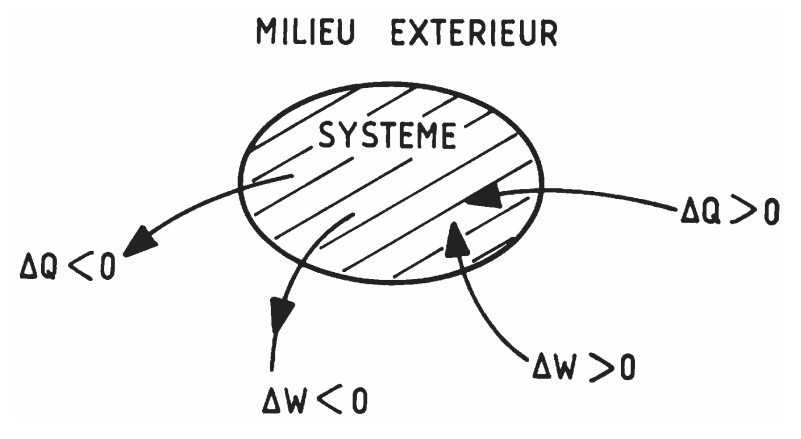
\includegraphics[width=0.4\linewidth]{../pic/3306/1.png}
\end{center}

Le premier principe se traduit par :
\[ \boxed{\Delta E = W + Q} \]
avec $\Delta E$ ne dépend que de l'état initial et final du système.\\
pour une transformation infinitésimale :
\[dE = \delta W + \delta Q\]

L'échange de travail $W$, ou de chaleur $Q$, dépend du chemin suivi par le système au cours de son évolution.
\subsubsection{Transformations quasi-statiques, réversibles et irréversibles}
Considérons un système effectuons une transformation , Si son évolution est telle qu'il reste toujours en équilibre thermodynamique la transformation est dite \underline{quasistatique}.\\
Si, de plus, par une simple inversion de la transformation on peut retrouver l'état initial, elle est \underline{réversible}.\\
Une transformation qui n'est pas réversible est dite \underline{irréversible}.
\subsection{Deuxième principe }
\subsubsection{Énoncé de Clausius}
\begin{center}\fbox{\begin{minipage}{\linewidth}  \center
			Il n'existe pas de processus dont le seul résultat soit de transférer de la chaleur d'un corps froid à un corps chaud.
		\end{minipage}}\end{center}
\subsubsection{Énoncé de Kelvin-Planck}
\begin{center}\fbox{\begin{minipage}{\linewidth}  \center
			Il n'existe pas de transformation dont le seul résultat soit de produire du travail à partir d'une seule source de chaleur à température constante.
		\end{minipage}}\end{center}
Cela signifie qu'il faut au moins deux sources à des températures différentes pour réaliser une conversion d'énergie calorifique en énergie mécanique.
\subsubsection{Les cycles de Carnot}
Les cycles de Carnot sont une suite cyclique de transformations quasi-statiques.\\
utilisant deux sources de chaleur aux températures $T_1$ et $T_2$, ($T_1 > T_2$).

\begin{minipage}{0.5\linewidth}
	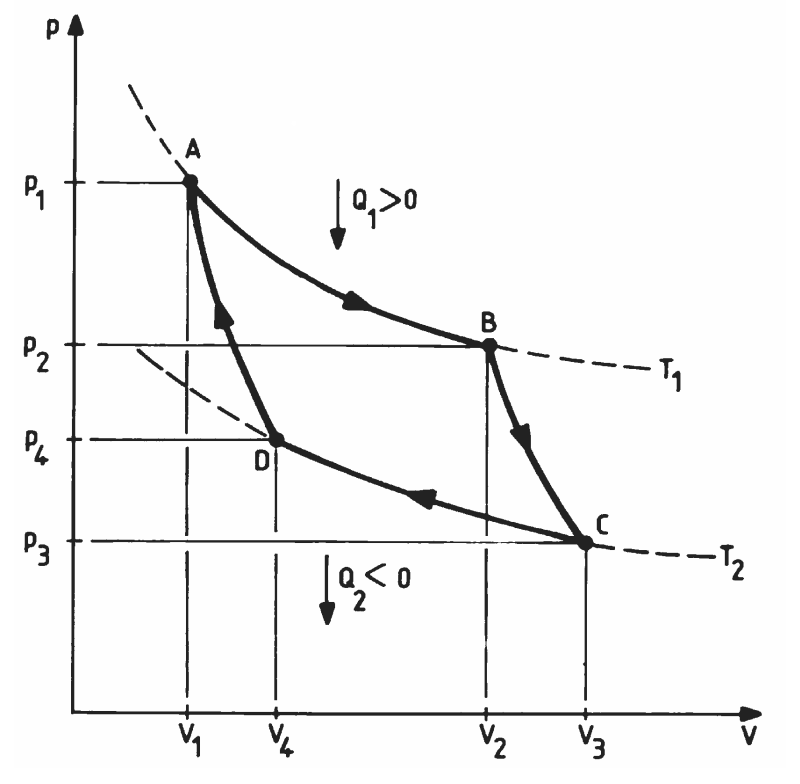
\includegraphics[width=\linewidth]{../pic/3306/2}
\end{minipage}
\begin{minipage}{0.5\linewidth}
	\begin{itemize}
		\item AB- isotherme réversible.
		\item BC- adiabatique réversible.
		\item CD- isotherme quasi-statique.
		\item DA- adiabatique réversible.
	\end{itemize}
\end{minipage}
Poserons $W_1' = -W_1$ et $Q_2' = -Q_2$.\\
D'après le premier principe :
\[\Delta E = W + Q = W_1 + W_2 + Q_1 + Q_2 = 0\]
\[W_1' - W_2 = Q_1 - Q_2'\]
Le rendement,$\eta$, du cycle est défini comme le rapport entre la quantité de travail fournie par le système et la quantité de chaleur prise à la source chaude.\\
Il vaut :
\[\eta = \frac{W_1' - W_2}{Q_1} = \frac{Q_1 - Q_2'}{Q_1} \]
Le cycle de Carnot permet de définir l'échelle de température absolue par la relation:
\[ \frac{Q_1}{Q_2'} = \frac{T_1}{T_2} \]
Cette équation peut être généralisée à tout cycle quasi-statique sous la forme:
\[ \oint \frac{\delta Q_{qs}}{T} = 0 \]
Cette équation constitue le théorème de Clausius.
\subsubsection{L'entropie}
Le théorème de Clausius nous permet d'introduire l'entropie par la relation :
\[\boxed{ dS = \frac{\delta Q_{qs}}{T} }\]
L'entropie est une fonction d'état, et une variable extensive.\\
L'entropie permet une autre formulation importante du second principe :
\begin{center}\fbox{\begin{minipage}{\linewidth}\center  L'entropie d'un système isolé ne peut qu'augmenter  \end{minipage}}\end{center}
\subsection{Troisième principe}
\begin{center}\fbox{\begin{minipage}{\linewidth}\center  L'entropie d'un solide ou d'un liquide pur en équilibre thermodynamique est nulle au zéro absolu.  \end{minipage}}\end{center}
\section{Fonctions thermodynamiques et conditions d'équilibre}
Considérons un système homogène de $r$ constituants ayant $N_1, N_2,..., N_r$ particules de type$ 1,2,...,r$.\\
L'énergie interne $E$ est une fonction des paramètres extensifs$ S, V, N_1,N_2,..., N_r$ :
\[E = E(S,V,N_1,...,N_r)\]
À chaque paramètre extensif correspond un paramètre intensif qui est, sauf pour la pression, égal à la dérivée partielle de $E$ par rapport à ce paramètre, les autres paramètres restant constants. \\
Dans le cas de la pression, il y a un signe moins:
\begin{itemize}
	\item Le paramètre intensif associé à l'entropie est la température :
	      \[(\frac{\partial E}{\partial S})_{V,N_1,...,N_r} = T\]
	\item Le paramètre intensif associé aux volume est la pression :
	      \[(\frac{\partial E}{\partial V})_{S,N_1,...,N_r} = -P\]
	\item Le paramètre intensif associé aux nombre de particules $N_j$ est le potentiel chimique $\mu_j$ :
	      \[(\frac{\partial E}{\partial N_j})_{S,V,N_1,...,N_{j-1},N_{j+1},...,N_r} = \mu_j\]
\end{itemize}
L'equation différentielle totale de l'énergie devient :
\[dE = (\frac{\partial E}{\partial S})_{V,N_1,...,N_r}dS + (\frac{\partial E}{\partial V})_{S,N_1,...,N_r} dV + \sum_{j=1}^{r} (\frac{\partial E}{\partial N_j})_{S,V,N_1,...,N_{j-1},N_{j+1},...,N_r} dN_j\]
\[\boxed{dE = TdS - PdV + \sum_{j=1}^{r}\mu_jdN_j}\]
Cette expression ne s'applique qu'aux transformations quasi-statiques. \\
Elle est aussi égale à :
\[dE = TdS - PdV = \delta Q + \delta W\]
L''expression suivant s'appelle la forme d'Euler de l'énergie interne.
\[ \boxed{E = TS - PV + \mu N} \]

Beaucoup d'expériences ont ainsi lieu à température et/ou à pression constante.\\
Lorsque c'est le cas, il est plus commode d'utiliser d'autres fonctions d'état pour étudier la thermodynamique du système.
\begin{itemize}
	\item Si l'on travaille a pression constante, on introduite l'enthalpie $H$:
	      \[ H = E + PV = TS + \sum_{j=1}^r\mu_jN_j \]
	      \[ \boxed{ dH = TdS + VdP + \sum_{j=1}^r\mu_jdN_j } \]
	\item Si l'on travaille a température constant, on introduit l'énergie libre $F$:
	      \[F = E-TS = -PV +\sum_{j=1}^r\mu_jN_j\]
	      \[ \boxed{ dF = -SdT -PdV + \sum_{j=1}^r\mu_jdN_j } \]
	\item Si l'on travaille a pression et temperature constants on introduit l'enthalpie libre $G$:
	      \[G = E + PV -TS = \sum_{j=1}^r\mu_jN_j\]
	      \[ \boxed{dG = -SdT + VdP + \sum_{j=1}^r\mu_jdN_j} \]
\end{itemize}
\chapter{LE MONDE MICROSCOPIQUE}
La physique statistique permet de faire la liaison entre les mondes macroscopiques et microscopiques.\\
Les caractéristique des constituants élémentaires au niveau microscopique :
\begin{itemize}
	\item Ils sont extrêmement petits(propriétés quantiques)
	\item Ils sont extrêmement nombreux (Leur évolution ne peut donc pas être traitée individuellement)
\end{itemize}
\section{Micro-états quantique}
Un micro-état est une configuration microscopique particulière d'un système.
\subsection{L'atome d'hydrogène}
Un atome d'hydrogène est un system constitué d'un proton et d'un électron qui interagissent par l'intermédiaire d'une force coulombienne attractive.\\
le proton est 1836 fois plus lourd que l'électron, alors en peut prendre l'approximation qu'il est immobile et que l'électron tourne autour de lui.\\
$E$ est l'énergie totale du system
\begin{itemize}
	\item Si $E \geq 0$, on a un  état de diffusion.\\
	      $E$ peut varier de façon continue et prendre toutes les valeurs possibles entre zéro et l'infini.
	\item Si $E \leq 0$, on a un état lié.\\
	      seules certaines valeurs de $E$ sont permises:
	      \[ \varepsilon_n = -\frac{13,6}{n^2}eV \]
	      $n$ est le nombre quantique principal.\\
	      L'état fondamental de l'atome d'hydrogène correspond à $n = 1$ et vaut $\varepsilon_1 =1 = -13, 6 eV$.\\
	      Les états d'énergie supérieure sont appelés états excités.\\
	      Pour un état d'énergie donnée, $\varepsilon_n$, on a plusieurs configurations possibles correspondant aux nombres quantiques $l, m, s, s_z$ qui obéissent aux lois suivantes :
	      \begin{itemize}
		      \item $ 0 \leq l \leq n-1$, $l$ est le nombre quantique secondaire.\\
		            Il est lié au moment angulaire orbital de l'électron.
		      \item $-l \leq m \leq m$, $m$ est le nombre quantique magnétique.\\
		            Il est lié à la projection du moment angulaire orbital sur l'axe z.
		      \item $s = \frac{1}{2}$,ce nombre quantique, que l'on appelle nombre quantique de spin, correspond à un degré de liberté purement interne de l'électron.
		      \item $- \frac{1}{2}\leq s_z \leq + \frac{1}{2}$. $s_z$ est le nombre quantique lié à la projection du spin sur l'axe z.\\
		            Ce nombre ne peut varier que par sauts d'une unité. Ici, il ne peut prendre que 2 valeurs : $\frac{1}{2}$ ou $\frac{-1}{2}$.
	      \end{itemize}
	      On définir un micro-état par un ensemble complet de nombres quantiques correspondant à des observables qui peuvent être mesurées simultanément(les opérateurs associés à ces grandeurs commutent).
	      \begin{itemize}
		      \item l'énergie.
		      \item le carré du moment angulaire orbital $L^2$.
		      \item Le projection du moment angulaire orbital sur l'axe z $L_z$.
		      \item Le carré du spin $s^2$.
		      \item Le projection du spin sur l'axe z $s_z$.
	      \end{itemize}
	      Ce choix particulier conduit à introduire l'ensemble des nombres quantiques $n, l, m, s $ et $ s_z$.
\end{itemize}
La donnée d'un ensemble complet de nombres quantiques ($n,l,m,s,s_z$) est nécessaire pour préciser exactement la configuration microscopique d'un système.\\
En effet, si cet ensemble est incomplet, on ne définit pas un micro-état mais une famille de micro-états.
\subsubsection{Dégénérescence}
Dans le cas où une même valeur de l'énergie correspond à plusieurs configurations, ou micro-états, on dit que le niveau est dégénéré.\\
Le degré de dégénérescence est le nombre de configurations associées à ce niveau d'énergie.\\
Par exemple, si $n =1,(\varepsilon_1)$  la dégénérescence est égale à 2 $(n = 1, l = 0, m = 0, s = \frac{1}{2} , s_z = \pm \frac{1}{2} )$, pour $n=2,\varepsilon_2$ il existe 8 micro-états.\\
\subsection{L'oscillateur harmonique à une dimension}
\subsubsection{Classiquement}
L'évolution d'un poids suspendu à un ressort autour de sa position d'équilibre, après qu'il en ait été légèrement écarté, représente un exemple d'oscillateur harmonique classique.\\
Supposons que le poids ait une masse m.\\
La position d'équilibre correspond a $x=0$.\\
Son énergie potentielle,$U$, est de la forme :
\[ U = \frac{1}{2}Kx^2 \]
avec $K$ une constante.\\
le corps est soumis a une force : $\frac{-\partial U}{\partial x} = -Kx$.\\
L'equation du mouvement s'écrite :
\[ m\frac{d^2x}{dt^2} = -Kx \]
La solution de cette équation est une sinusoïde dont la pulsation $w$ est donnée par:$w = \sqrt{\frac{K}{m}}$.\\
Classiquement, toutes les valeurs positives de l'énergie sont permises.
\subsubsection{Au niveau microscopique}
Un exemple très simple est donné par la molécule d'hydrogène dont les deux atomes peuvent osciller le long de l'axe de symétrie de la molécule.\\
Les niveaux d'énergie et du pulsation sont quantifiés.\\
les niveaux d'énergie sont donnés par l'expression :
\[ \varepsilon_n = (n + \frac{1}{2})\hbar w \]
\begin{center}
	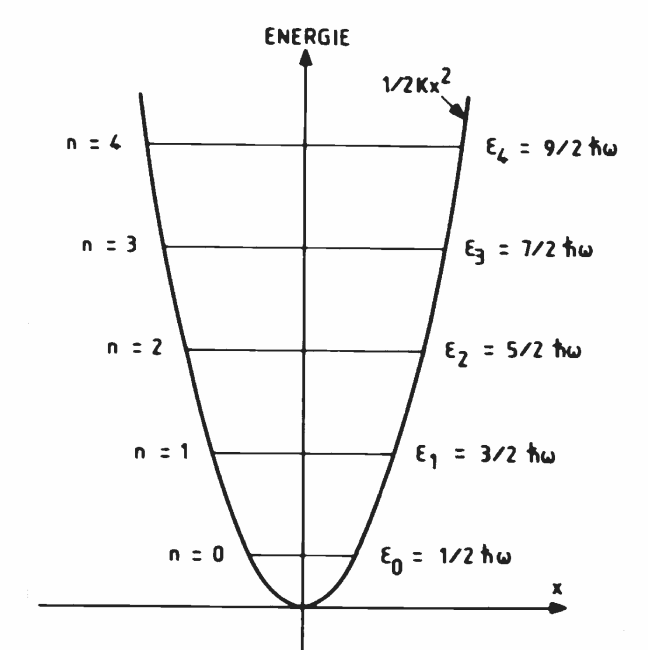
\includegraphics[width=0.5\linewidth]{../pic/3306/3.png}
\end{center}
\subsection{Une particule libre dans une boîte cubique}
\begin{center}
	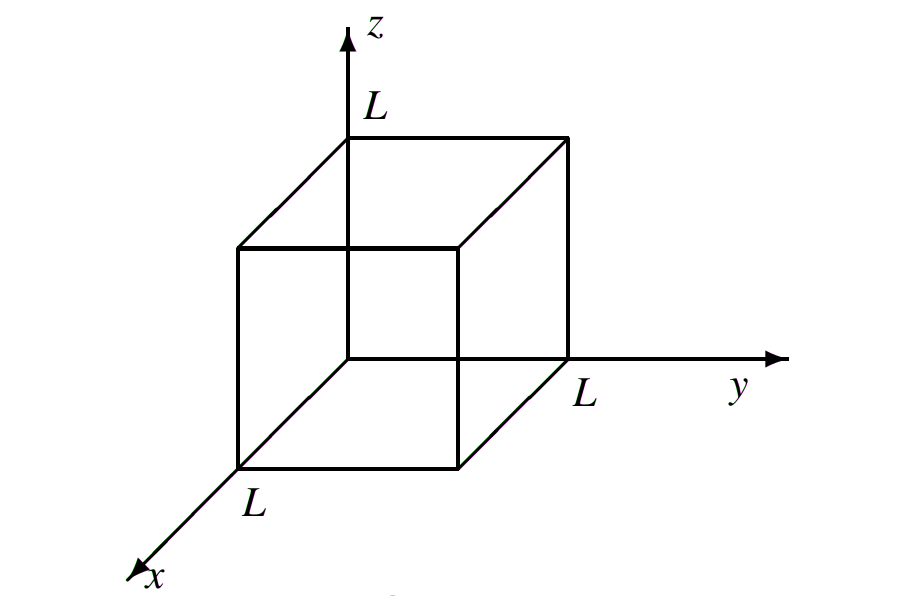
\includegraphics[width=0.5\linewidth]{../pic/3306/4.png}
\end{center}
Une particule libre, de masse $m$ et de spin nul, placée dans une boîte cubique de coté $L$.\\
L'énergie potentielle de ce système est nulle à l'intérieur de la boîte et infiniment répulsive ($U = +\infty$) à l'extérieur.\\
Seules certaines valeurs d'énergie sont permises :
\[ \varepsilon_{n_x n_y n_z} = \frac{\pi^2\hbar^2}{2mL^2}(n_x^2 + n_y^2 + n_z^2) \]
avec $n_x,n_y$ et $n_z$ sont les nombres quantiques associés à chacune des directions de l'espace : x, y et z.\\
Posons : $\varepsilon_0 = \frac{\pi^2\hbar^2}{2mL^2} \implies \varepsilon_{n_x n_y n_z} = \varepsilon_0(n_x^2 + n_y^2 + n_z^2)$\\
L'état fondamental correspond à $n_x = n_y = n_z = 1$ et son énergie vaut $\varepsilon_{111} = 3\varepsilon_0$. Il n'est pas dégénéré.\\
Le premier état excité peut être construit de 3 manières différentes:\\
$\begin{cases}
		\varepsilon_{211} =6\varepsilon_0 : n_x =2, n_y = 1, n_z =1 \\
		\varepsilon_{121} =6\varepsilon_0 : n_x =1, n_y = 2, n_z =1 \\
		\varepsilon_{112} =6\varepsilon_0 : n_x =1, n_y = 1, n_z =2
	\end{cases}$
\subsection{Les systèmes à $N$ particules}
Les systèmes réels sont complexes car ils comportent un nombre élevé,$N$, de particules identiques.\\
Dans le cas le plus général, les $N$ particules ont des interactions entre elles qui mettent en jeu deux ou même plusieurs particules.\\

Par exemple, le cas pour un ensemble de $N$ électrons. Chacun d'entre eux interagit avec les $N - 1$ autres par l'intermédiaire de la force de Coulomb.\\

On peut aussi avoir des interactions plus complexes : c'est le cas des nucléons dans le noyau.\\
l'énergie totale d'un tel système n'est pas égale à la somme des énergies associées à chaque particule car il n'est pas possible de séparer l'énergie potentielle totale en contributions individuelles associées à chaque particule et ne dépendant que de la position de celle-ci.\\

Il arrive parfois que les interactions complexes entre les particules se traduisent, avec une bonne approximation, par un potentiel moyen.\\
Dans une telle situation, le problème se simplifie beaucoup car il suffit de considérer que chaque particule évolue dans ce potentiel moyen sans interaction avec les autres particules.\\
On peut alors encore de parler d'états individuels.\\
L'interaction entre les électrons peut se traduire approximativement par un potentiel moyen.
\section{Bosons et Fermions}
\subsection{Definitions}
Au niveau microscopique les particules sont indiscernables.\\
Toutes les particules de la nature ont un spin s qui est soit entier soit demi-entier.\\
les bosons (comme l'électron) si s est entier, et les fermions (comme le photon) s'il est demi-entier.\\
\begin{itemize}
	\item La fonction d'onde d'un système constitué de plusieurs fermions est antisymétrique par rapport à l'échange de deux particules.\\
	      Cette propriété implique que deux particules ne peuvent pas être dans le même état quantique.\\
	      C'est ce que l'on appelle le principe d'exclusion de Pauli.
	\item La fonction d'onde d'un système de bosons doit être symétrique par rapport à l'échange de deux particules.\\
	      Plusieurs bosons peuvent se trouver dans la même configuration quantique.\\
	      On dit qu'ils obéissent à la statistique de Bose-Einstein.
\end{itemize}
\subsection{Micro-état et spin}
Soit une particule libre dans une boîte cubique et ait un spin $s$.\\
Dans ce cas il est nécessaire d'introduire deux nombres quantiques supplémentaires : $s$ et $s_z$.
\begin{itemize}
	\item Pour une particule de spin nul, les micro-états sont complètement déterminés par la simple donnée de $n_x, n_y et n_z$
	\item Lorsque le spin de la particule est différent de zéro il faut préciser les valeurs de $s$ et $s_z$.\\
	      Par exemple, si $s= 1$,et pour $n_x,n_y$ et $n_z$ fixes, on peut définir trois micro-états:\\
	      $\begin{cases}
			      n_x,n_y,n_z,1,-1 \\
			      n_x,n_y,n_z,1,0  \\
			      n_x,n_y,n_z,1,1
		      \end{cases}$
\end{itemize}
\subsubsection{Une particule libre}
Considérons une particule libre, de spin s, dans une boîte cubique.\\
Supposons que son énergie soit égale à $12\varepsilon_0 (n_x = n_y = n_z = 2)$.\\
Pour une particule sans spin, cet état d'énergie n'est pas dégénéré et correspond à une seule configuration.
\begin{itemize}
	\item Si $s = 0 \to (2,2,2,0,0)$
	\item Si $s = \frac{1}{2} \to (2,2,2,\frac{1}{2},\frac{-1}{2})$ et $(2,2,2,\frac{1}{2},\frac{1}{2})$
	\item Si $s = \frac{3}{2}$,$s_z$ peut prendre $2s + 1 =4 \to \begin{cases}
			      \textstyle(2,2,2,\frac{3}{2},\frac{-3}{2}) \\
			      \textstyle(2,2,2,\frac{3}{2},\frac{-1}{2}) \\
			      \textstyle(2,2,2,\frac{3}{2},\frac{1}{2})  \\
			      \textstyle(2,2,2,\frac{3}{2},\frac{3}{2})  \\
		      \end{cases}$
\end{itemize}
\subsubsection{Deux particules libres}
Considérons deux particules libres, de spin s, dans une boîte cubique.\\
Supposons que son énergie soit égale à $15\varepsilon_0$.\\
Une des particules soit sur le niveau $3\varepsilon_0$ et l'autre sur le niveau $12\varepsilon_0$,ou par la combinaison $9\varepsilon_0$ et $6\varepsilon_0$.\\
Un micro-état associé à ce système de deux particules est déterminé par la donnée de 10 nombres quantiques $(n_{x_1},n_{y_1},n_{z_1},s_1,s_{z_1},n_{x_2},n_{y_2},n_{z_2},s_2,s_{z_2})$.\\
\begin{itemize}
	\item Pour $s=0 \to (1,1,1,0,0,2,2,2,0,0)$
	\item Pour $s = \frac{1}{2} \to \begin{cases}
			      \textstyle(1,1,1,\frac{1}{2},\frac{-1}{2},2,2,2,\frac{1}{2},\frac{-1}{2}) \\
			      \textstyle(1,1,1,\frac{1}{2},\frac{-1}{2},2,2,2,\frac{1}{2},\frac{1}{2})  \\
			      \textstyle(1,1,1,\frac{1}{2},\frac{1}{2},2,2,2,\frac{1}{2},\frac{1}{2})   \\
			      \textstyle(1,1,1,\frac{1}{2},\frac{1}{2},2,2,2,\frac{1}{2},\frac{-1}{2})  \\
		      \end{cases}$
\end{itemize}
\section{Systèmes a N particules indépendantes}
\subsection{Particules discernables}
Supposons qu'une particule soit bleue (B), l'autre rouge (R) et la dernière jaune (J).\\
Cherchons de combien de manières différentes trois particules peuvent conduire à 3 unités d'énergie.
\begin{itemize}
	\item Une particule sur le niveau 3 et deux sur le niveau zéro.
	\item Une particule sur chacun des trois premiers niveaux.
	\item Trois particules sur le premier niveau.
\end{itemize}
Nous noterons un micro-état par ($n_B$, $n_R$, $n_J$) où $n_B,n_R$ et $n_J$ repèrent les niveaux occupés par les particules B, R et J.\\

\begin{minipage}{0.6\linewidth}
	\begin{itemize}
		\item Pour la première configuration nous avons trois micro-états possibles.
		\item Pour la deuxième configuration nous avons 6 micro-états possibles.
		\item Pour la troisième configuration nous avons 1 micro-état possible.
	\end{itemize}
\end{minipage}
\begin{minipage}{0.4\linewidth}
	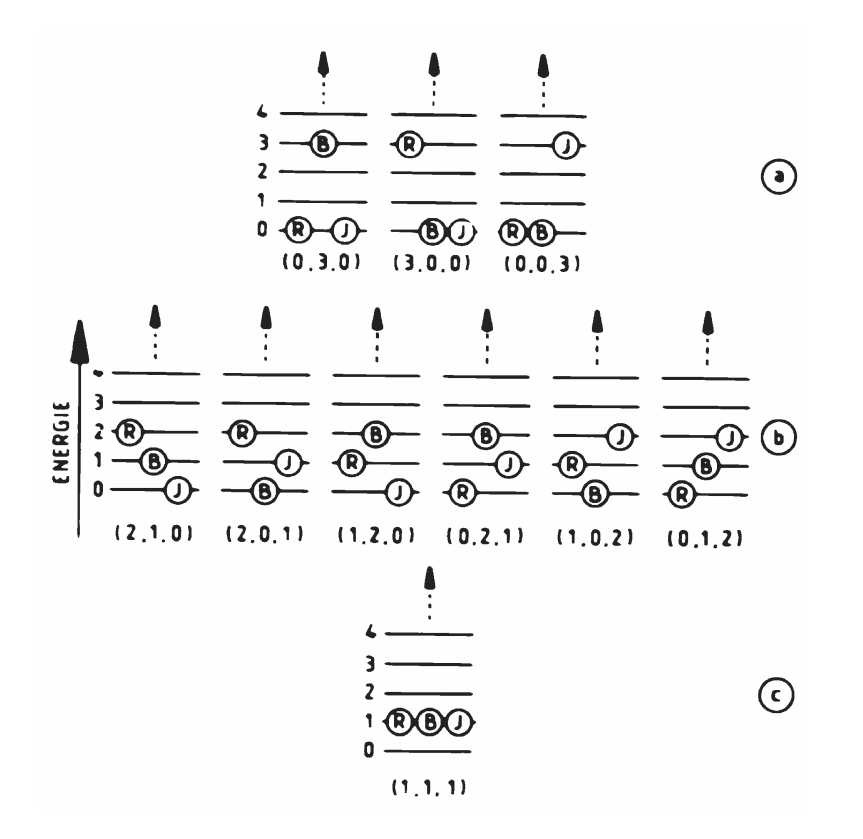
\includegraphics[width=\linewidth]{../pic/3306/6}
\end{minipage}
Au total, pour ce système à trois particules, la dégénérescence du niveau d'énergie est égale à 10 et nous avons 10 micro-états différents à trois particules.
\subsection{Particules indiscernables}
\subsubsection{Bosons}
\begin{minipage}{0.7\linewidth}
	Supposons que les trois particules soient des bosons de spin nul.\\
	Il n'y a pas de restriction pour l'occupation des niveaux à une particule.\\
	Nous n'avons au total que trois micro-états.
\end{minipage}
\begin{minipage}{0.3\linewidth}
	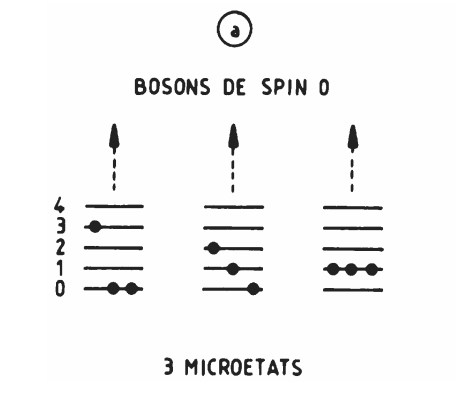
\includegraphics[width=\linewidth]{../pic/3306/7}
\end{minipage}
\subsubsection{Fermions}

\begin{minipage}{0.8\linewidth}
	Supposons que les trois particules soient des fermions de spin $\frac{1}{2}$.\\
	Le principe d'exclusion de Pauli empêche deux fermions d'avoir les mêmes nombres quantiques.\\
	la configuration où l'on a trois particules dans l'état 1 est impossible.

\end{minipage}
\begin{minipage}{0.2\linewidth}
	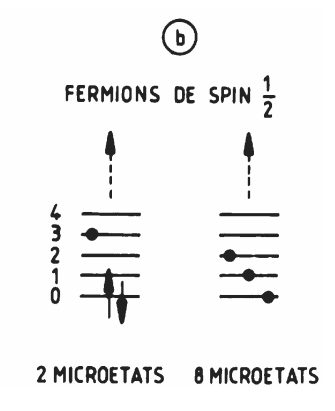
\includegraphics[width=\linewidth]{../pic/3306/8}
\end{minipage}
\section{Micro-état et macro-états}
Un macro-état est complètement déterminé si l'on connaît 2 paramètres macroscopiques (P et T par exemple).\\
Il faudrait connaître 3N nombres quantiques pour déterminer un micro-état.\\
Soit $\Omega(E)$ est le nombre de micro-états accessibles au système lorsque son énergie totale est égale à $E$.\\
Un système à $N$ particules a $f = 3N$ degrés de liberté.\\
On peut montrer que le nombre de micro-états varie très approximativement comme:
\[\Omega(E)\approx E^f\]
Remarque :
\push{
	Les particules de la nature sont soit des bosons, soit des fermions.\\
	Cette distinction n'est importante que lorsque le système a un comportement quantique.
}
\section{L'espace de phase}
Considérer un système constitué d'une particule de masse $m$.\\
Au temps $t$ il est possible de calculer la position $r$ de la particule et son impulsion $p$ si l'on connaît :
\begin{itemize}
	\item Les forces auxquelles elle est soumise en chaque point de l'espace.
	\item Sa position $r_0$ et son impulsion $p_0$ au temps $t = 0$.
\end{itemize}
Dans le cas d'une force dérivant d'un potentiel $U$:
\[ \frac{dp}{dt} = - \frac{\partial U}{\partial r} = -\nabla U \]
$p$ est défini par l'équation:
\[ \frac{dr}{dt} = \frac{p}{m} \]
\underline{L'espace de phase} de la particule est un espace cartésien à six dimensions dont les axes sont associés aux variables $x, y, z, p_x, p_y et p_z$.
\begin{center}
	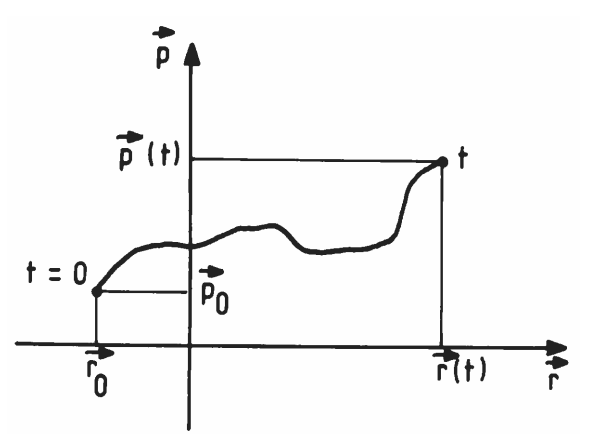
\includegraphics[width=0.3\linewidth]{../pic/3306/9.png}
\end{center}
\subsection{Trajectoire d'oscillateur harmonique}
Étudions la trajectoire dans l'espace de phase associée à un oscillateur harmonique à une dimension dont l'énergie totale est égale à $E$.\\
une masse $m$ suspendue à un ressort dont la rigidité est égale à $K$.\\
l'énergie totale est :
\[ E = \frac{p^2}{2m} + \frac{1}{2}Kq^2 \]
$p$ et $q$ désignent respectivement l'impulsion et la coordonnée.\\
Cette equation est une ellipse dont les demi-axes sont respectivement $\sqrt{2mE}$ et $\sqrt{\frac{2E}{K}}$.\\

L'énergie du système est comprise entre $E$ et $E + \delta E$.\\
Les trajectoires dans l'espace de phase seront donc toutes comprises entre deux surfaces d'énergie:
\[E + \delta E = \frac{p^2}{2m} + \frac{1}{2}Kq^2 \]
\begin{center}
	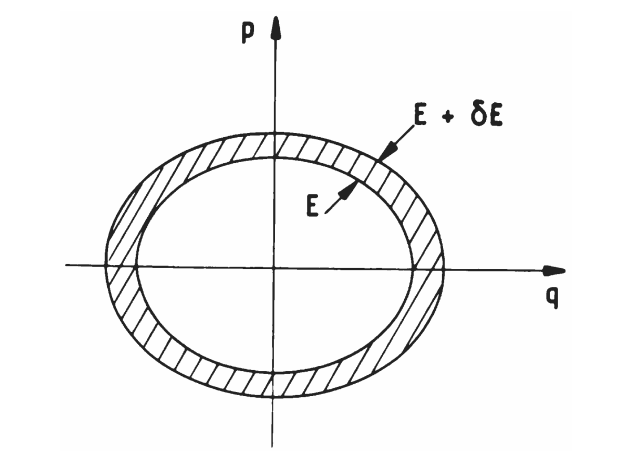
\includegraphics[width=0.4\linewidth]{../pic/3306/10.png}
\end{center}

\subsection{A N particules}
La généralisation à un système à $N$ particules est immédiate.\\
La configuration d'un tel système est déterminée si l'on connaît $3N$ positions et $3N$ impulsions.\\
L'espace de phase a donc $6N$ dimensions.\\
La dimension de l'espace de phase est égale à $2f$.\\

Au cours de son évolution, le système décrit une trajectoire dans cet espace, deux trajectoires ne peuvent se couper.
\section{Micro-État classique}
\subsection{Configurations et micro-états classiques}
Si nous voulons développer une physique statistique classique, il faut retrouver, pour une énergie totale donnée, le même nombre de micro-états classiques que dans l'approche quantique.\\
la mécanique classique prévoit une infinité de configurations puisque les variables de l'espace de phase peuvent varier de manière continue.\\
Par exemple pour un oscillateur harmonique il y a une infinité de points (configurations) compris entre les ellipses associées à $E $ et $E +\delta E$.\\
A un système à $f$ degrés de liberté on subdivise l'espace de phase en cellules élémentaires de côté $\delta q$, pour les coordonnées $q_i$, et $\delta p$, pour les coordonnées $p_i$.\\
Chacune de ces cellules, dont le volume est égal à $(\delta q \delta p)^f$, est associée à un micro-état classique.\\
Soit $V$ est le volume accessible au système lorsque son énergie est comprise entre $E$ et $E + \delta E$.\\
\underline{Le nombre de micro-états classiques accessibles au système est égal à :}
\[\boxed{\frac{V}{(\delta q \delta p)^f}}\]
A une dimension pour $V = S = \delta q \delta p$ et $f =1$:
\begin{center}
	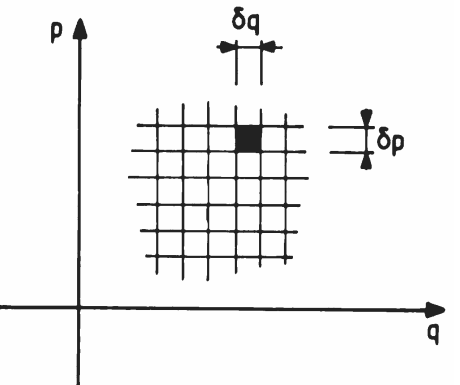
\includegraphics[width=0.3\linewidth]{../pic/3306/11.png}
\end{center}
\underline{La plus petite cellule de l'espace de phase compatible avec les lois de la mécanique quantique est pour :}
\[\boxed{\delta q \delta p = h}\]
$\implies $ Le nombre de micro-états classiques accessibles au système est égal à $\frac{V}{h^f}$
\subsection{Micro-états classiques et spin}
Pour tenir compte du spin $s$, on introduit une dégénérescence additionnelle égale à $2s +1$(égale a deux seulement dans le cas des photons).\\
Le nombre total de micro-états classiques est alors égal a :
\[ \boxed{ (2s +1) \frac{V}{h^f} } \]
\section{Travail et Chaleur a l'échelle microscopique}
Soit $N$ particules indépendantes dans une boîte cubique de côté $L$.\\
Le volume de cette boîte vaut $L^3$.\\
\subsubsection{Travail}
Le travail mécanique correspond à une variation du volume V du système.\\
Les niveaux d'énergie à une particule sont donnés par :
\[ \varepsilon_{n_x,n_y,n_z} = \frac{\pi^2 \hbar^2}{2mL^2}(n_x^2 + n_y^2 + n_z^2) = \frac{\pi^2 \hbar^2}{2mV^{\frac{2}{3}}}(n_x^2 + n_y^2 + n_z^2) \]
D'après l'equation :
\begin{itemize}
	\item Si $V$ diminue les niveaux d'énergie s'espacent.
	\item Si $V$ augment les niveaux d'énergie se rapprochent.
\end{itemize}
\begin{center}
	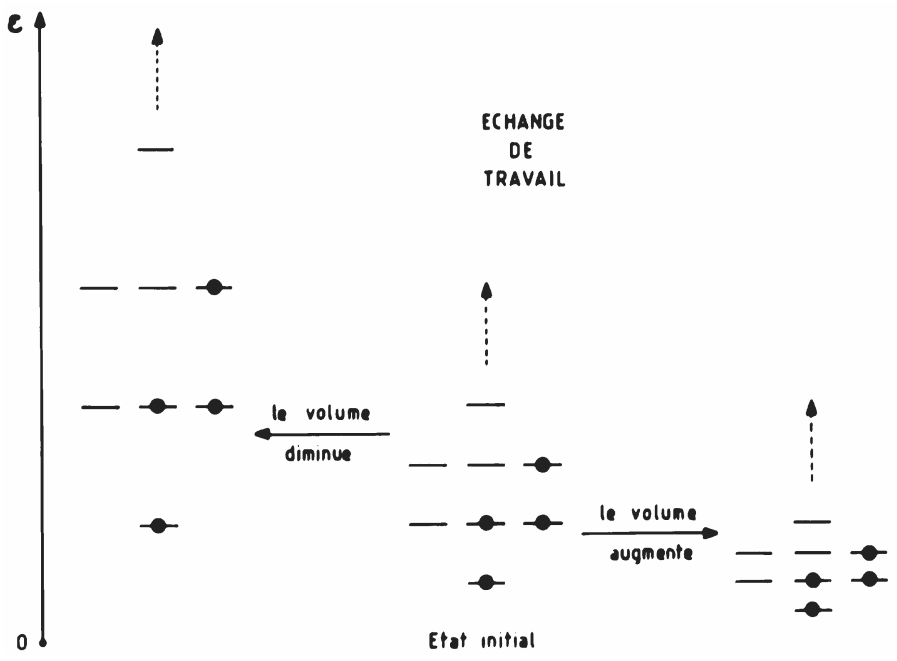
\includegraphics[width=0.5\linewidth]{../pic/3306/12.png}
\end{center}
Un transfert d'énergie mécanique se traduit donc par un changement des niveaux d'énergie sans changement de l'occupation de ceux-ci par les particules.\\
Le travail mécanique est un transfert d'énergie au niveau macroscopique puisqu'on l'obtient par changement d'un paramètre externe.
\subsubsection{Chaleur}
Supposons à présent que le volume reste constant.\\
Les niveaux d'énergie sont fixés et il n'y a pas d'échange d'énergie mécanique.\\
Par contre, on peut changer l'occupation des niveaux à une particule.\\
Ceci se traduit par une variation d'énergie du système et correspond à \underline{un échange de chaleur}.
\begin{center}
	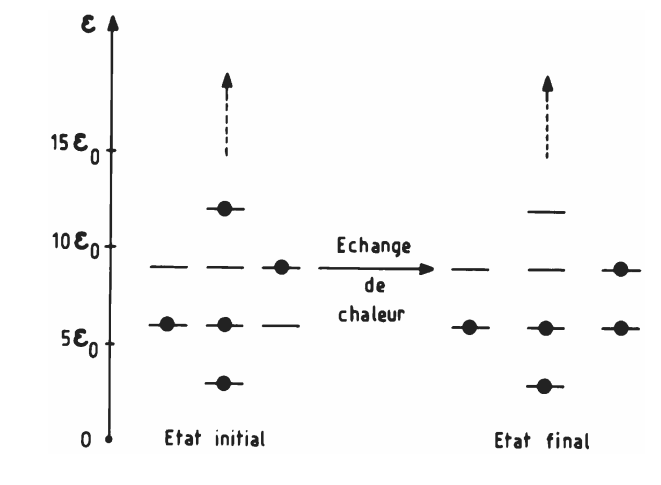
\includegraphics[width=0.4\linewidth]{../pic/3306/13.png}
\end{center}
la chaleur est un transfert d'énergie au niveau microscopique car elle correspond à un changement d'occupation des niveaux de particule individuelle.
\chapter{POSTULATS DE LA PHYSIQUE STATISTIQUE}
\section{Énoncé des postulats }
\subsection{Postulat 1}
\begin{center}
	Tous les micro-états accessibles à un système isolé en équilibre sont équiprobables.
\end{center}
La probability pour qu'il soit dans un micro-état donné est égal a $\frac{1}{\Omega(E)}$
\subsection{Postulat 2}
\begin{center}
	La moyenne dans le temps d'un paramètre quelconque est égale à la moyenne de ce paramètre prise sur un ensemble de systèmes.
\end{center}
Pour expliciter un peu plus le second postulat de la physique statistique, plaçons-nous dans le cadre de la mécanique classique et considérons une grandeur macroscopique quelconque $y$ associée à un système de $N$ particules.\\
Cette grandeur dépend des coordonnées $q_i$ et des impulsions $p_i$ de chaque particule.\\
Elle dépend donc du temps $t$ car les coordonnées et les impulsions sont des fonctions du temps.\\
La moyenne dans le temps de la grandeur y est définie par :
\[ \moyenne{y}_t = \lim_{t'\to \infty}\frac{1}{t'}\int^{t'}_0y(t')dt' \]
Considérons un ensemble $\{ \varepsilon \}$ de $N$ systèmes au temps t. \\
La moyenne de la variable $y$, pris sur l'ensemble $\{ \varepsilon \}$, est égal a :
\[ \moyenne{y} = \frac{1}{N}\sum_{i=1}^N y_i(t) \]
avec $y_i(t)$ est la valeur de $y(t)$ pour le système $i$ appartenant a l'ensemble $\{ \varepsilon \}$.\\
Le second postulat pose que
\[\moyenne{y}_t = \moyenne{y}\]
\section{L'entropie statistique}
Pour un système en équilibre L'entropie statistique :
\[ S = k \log(\Omega(E)) \]
Avec $\begin{cases}
		k : \text{ est le constant de boltzmann} \\
		\Omega(E) : \text{le nombre de micro-etats accessibles a la système dont l'energie est egal a E }
	\end{cases}$
\section{Notions de théorie de l'information }
\subsection{L'information}
L'information est une quantité liée à la connaissance d'une situation.\\
Soit une boule dans $N$ boites identiques.\\
Nous allons introduire une quantité $I$ qui va nous permettre de chiffrer le manque d'information sur le système.\\
Il est clair que $I$ doit être une fonction de $N$.\\
Si le nombre de boîtes augmente, l'information sur le système va diminuer:
\[ I(M) > I(N) \text{ si } M > N \]
Supposons à présent que chacune des boîtes soit divisée en $M$ compartiments équiprobables.\\
Il y a au total $NM$ compartiments équiprobables.\\
L'additivité de l'information manquante s'exprime par :
\[ I(MN) = I(M) + I(N) \]
Nous appellerons l'information manquante : L'entropie d'information
\[ I = -k\sum_{i=1}^N P_i\log(P_i) \]
Avec $P_i$ sera la probabilité d'occuper un micro-état.\\
Si $P_i = \frac{1}{N}$, toutes les configurations sont équiprobables et $I = k\log(N)$.\\
On note que L'équilibre statistique est atteint lorsque tous les micro-états accessibles sont équiprobables ,lorsque $P_i = \frac{1}{\Omega(E)}$.\\
Dans ce cas : $I = S = k\log(\Omega(E))$
\subsection{Entropie et théorie de l'information}
A partir de la théorie de l'information en remplaçant le premier postulat par l'énoncé suivant :
\begin{center}
	L'information sur un système en équilibre est minimum.
\end{center}
\[ S = -k\sum_{i\in M} P_i\log(P_i) \]
la loi du maximum de l'entropie, à $E$ fixée, est équivalente à avoir le minimum d'information sur le système.
\section{Irréversibilité}
Considérons un système isolé en équilibre statistique dont l'état macroscopique est déterminé par un ensemble de contraintes externes.\\
Soit $\Omega_i$ le nombre de micro-états accessibles à ce système.\\
Soit $\Omega_f$ le nombre de micro-états accessibles dans l'état final lorsque les contraintes ont été enlevées.\\
\begin{itemize}
	\item Si $\Omega_f > \Omega_i$ la transformation est irréversible car même si on rétablit les contraintes, on ne reviendra pas dans la situation initiale.
	      \begin{center}
		      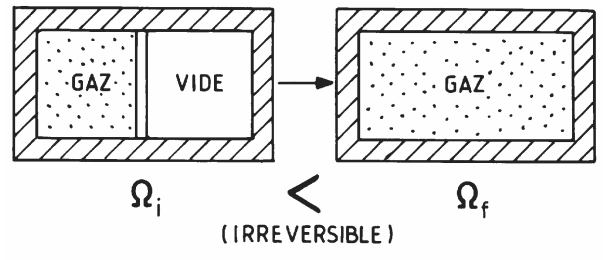
\includegraphics[width=0.5\linewidth]{../pic/3306/14.png}
	      \end{center}
	\item Si $\Omega_f = \Omega_i$ la transformation est réversible. Si l'on remet les contraintes sur le système on revient dans l'état initial.
	      \begin{center}
		      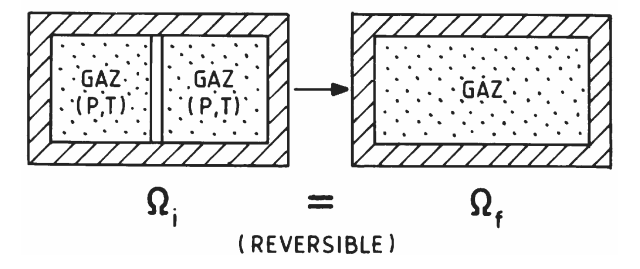
\includegraphics[width=0.5\linewidth]{../pic/3306/15.png}
	      \end{center}
\end{itemize}
Une transformation réversible se fait donc à entropie constante puisque le nombre de micro-états ne change pas.\\
Si, à chaque étape de l'évolution du système, celui-ci passe par une séquence d'états en équilibre statistique, la transformation est dite quasi-statique.
\section{Valeurs moyennes et fluctuations}
considérons un système de quatre fermions de spin $s = \frac{1}{2}$.\\
le système de quatre fermions ait une énergie totale égale à 5.\\
On néglige d'abord le spin,les configurations à quatre particules conduisant à une énergie totale égale à 5:
\[   \begin{matrix}
		5=5+0+0+0 & 5=4+1+0+0 & 5 = 3+2+0+0 \\
		5=3+1+1+0 & 5=2+2+1+0 & 5 = 2+1+1+1 \\
	\end{matrix} \]
Tenons compte maintenant du spin les fermions obéissent au principe de Pauli et on ne peut pas mettre plus de deux particules sur chaque niveau de particule individuelle car le spin est égal à $\frac{1}{2}$\\
Le configuration devient
\[   \begin{matrix}
		5=4+1+0+0 & 5 = 3+2+0+0 \\
		5=3+1+1+0 & 5=2+2+1+0   \\
	\end{matrix} \]
Les 4 configurations possibles correspondent toujours à deux particules sur des niveaux différents et deux sur un troisième.\\
Pour le niveau qui contient deux particules,les spins sont appariés.\\
Par contre, pour les deux particules qui se trouvent sur des niveaux différents,nous avons le choix entre deux possibilités $(s_z = \pm\frac{1}{2})$\\
Nous allons maintenant nous intéresser à la projection $S_z$ du spin total de cet ensemble de fermions.\\
$S_z$ peut varier de $-2$ a $+2$ par sauts d'un unité.\\
Les deux valeurs extrêmes, -2 et +2, sont obtenues lorsque le spin des quatre particules sont alignés parallèlement ou anti-parallèlement à l'axe $z$.
\begin{center}
	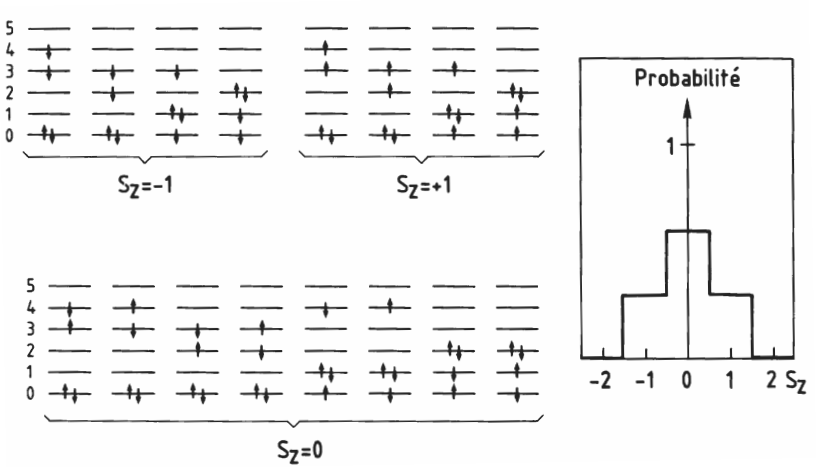
\includegraphics[width=0.5\linewidth]{../pic/3306/16.png}
\end{center}
$50\%$ des cas on obtient un système de l'ensemble avec $S_z = 0$ et que dans $0\%$ des cas on a $S_z = \pm 2$.\\
La valeur la plus probable est $\tilde{S_z} = 0$.\\
La valeur moyenne $\moyenne{S_z}$ est également nulle.\\
L'existence d'un distribution de probabilité implique que le résultat d'une mesure est incertain.\\
Un résultat est plus probable que l'autres mais il existe une dispersion autour de cette valeur.\\
Cette dispersion constitue ce que l'on appelle des fluctuations.\\

Pour les systèmes macroscopiques, la distribution de probabilité d'une variable macroscopique, y, est extrêmement piquée et les fluctuations autour de la valeur la plus probable, y, sont extrêmement faibles.
\section{QUELQUES DISTRIBUTIONS IMPORTANTES}
\subsection{La distribution binomiale}
Nous allons traiter le problème d'un système dont l'évolution au cours du temps se fait par étapes discrètes et aléatoires dans un espace à une dimension.\\
À chaque étape,le système avance d'une longueur l donnée dans l'une ou l'autre direction.\\
Chaque pas est supposé indépendant du précédent.\\
La probabilité d'aller à gauche est $p$,à droite $q = 1-p$.\\
\begin{center}
	Apres N étapes, nous voudrions savoir à quelle distance il se trouve de l'origine.
\end{center}
On  introduire une distribution de probabilité : \underline{la distribution binomiale}.
Nous voulons calculer la probabilité pour que le système soit à la distance x de l'origine.
\[x =ml , m \text{ est un entier tel que:} -N\leq m \leq +N\]
Les bornes $-N$ et $+N$ correspondent a la distance maximum qu'il peut parcourir dans une direction.\\
la fonction de distribution de probabilité $P(m)$ pour chaque valeur de $m$ appartenant a l'intervalle.\\
$n$ le nombre de pas vers la droit et $n'$ le nombre de pas vers la gauche, on a $N = m + n$.\\
La probabilité d'avoir une sequence particulier correspondant a $n$ pas a droite et $n'$ pas a gauche est égal a $p^nq^{n'}$.\\
Le résultat correspond au nombre de combinaisons de $N$ objets pris $n$ a $n$:
\[ C^n_N=\frac{N!}{n!(N-n)!}=\frac{N!}{n!n'!} \]
La probabilité $P(n)$ d'avoir $n$ pas vers la droite est donc :
\[P(n) = \frac{N!}{n!n'!}p^np^{n'}\]
que l'on peut aussi écrire sous la forme:
\[P(n) = C^n_Np^nq^{N-n}\]





\end{document}